\documentclass[twoside]{book}

% Packages required by doxygen
\usepackage{calc}
\usepackage{doxygen}
\usepackage{graphicx}
\usepackage[utf8]{inputenc}
\usepackage{makeidx}
\usepackage{multicol}
\usepackage{multirow}
\usepackage{textcomp}
\usepackage[table]{xcolor}

% Font selection
\usepackage[T1]{fontenc}
\usepackage{mathptmx}
\usepackage[scaled=.90]{helvet}
\usepackage{courier}
\usepackage{amssymb}
\usepackage{sectsty}
\renewcommand{\familydefault}{\sfdefault}
\allsectionsfont{%
  \fontseries{bc}\selectfont%
  \color{darkgray}%
}
\renewcommand{\DoxyLabelFont}{%
  \fontseries{bc}\selectfont%
  \color{darkgray}%
}

% Page & text layout
\usepackage{geometry}
\geometry{%
  a4paper,%
  top=2.5cm,%
  bottom=2.5cm,%
  left=2.5cm,%
  right=2.5cm%
}
\tolerance=750
\hfuzz=15pt
\hbadness=750
\setlength{\emergencystretch}{15pt}
\setlength{\parindent}{0cm}
\setlength{\parskip}{0.2cm}
\makeatletter
\renewcommand{\paragraph}{%
  \@startsection{paragraph}{4}{0ex}{-1.0ex}{1.0ex}{%
    \normalfont\normalsize\bfseries\SS@parafont%
  }%
}
\renewcommand{\subparagraph}{%
  \@startsection{subparagraph}{5}{0ex}{-1.0ex}{1.0ex}{%
    \normalfont\normalsize\bfseries\SS@subparafont%
  }%
}
\makeatother

% Headers & footers
\usepackage{fancyhdr}
\pagestyle{fancyplain}
\fancyhead[LE]{\fancyplain{}{\bfseries\thepage}}
\fancyhead[CE]{\fancyplain{}{}}
\fancyhead[RE]{\fancyplain{}{\bfseries\leftmark}}
\fancyhead[LO]{\fancyplain{}{\bfseries\rightmark}}
\fancyhead[CO]{\fancyplain{}{}}
\fancyhead[RO]{\fancyplain{}{\bfseries\thepage}}
\fancyfoot[LE]{\fancyplain{}{}}
\fancyfoot[CE]{\fancyplain{}{}}
\fancyfoot[RE]{\fancyplain{}{\bfseries\scriptsize Generated on Mon Mar 6 2017 20\-:30\-:23 for Proyecto\-: Distancia entre texto utilizando autómata de Levenshtein by Doxygen }}
\fancyfoot[LO]{\fancyplain{}{\bfseries\scriptsize Generated on Mon Mar 6 2017 20\-:30\-:23 for Proyecto\-: Distancia entre texto utilizando autómata de Levenshtein by Doxygen }}
\fancyfoot[CO]{\fancyplain{}{}}
\fancyfoot[RO]{\fancyplain{}{}}
\renewcommand{\footrulewidth}{0.4pt}
\renewcommand{\chaptermark}[1]{%
  \markboth{#1}{}%
}
\renewcommand{\sectionmark}[1]{%
  \markright{\thesection\ #1}%
}

% Indices & bibliography
\usepackage{natbib}
\usepackage[titles]{tocloft}
\setcounter{tocdepth}{3}
\setcounter{secnumdepth}{5}
\makeindex

% Custom commands
\newcommand{\clearemptydoublepage}{%
  \newpage{\pagestyle{empty}\cleardoublepage}%
}


%===== C O N T E N T S =====

\begin{document}

% Titlepage & ToC
\pagenumbering{roman}
\begin{titlepage}
\vspace*{7cm}
\begin{center}%
{\Large Proyecto\-: Distancia entre texto utilizando autómata de Levenshtein }\\
\vspace*{1cm}
{\large Generated by Doxygen 1.8.6}\\
\vspace*{0.5cm}
{\small Mon Mar 6 2017 20:30:23}\\
\end{center}
\end{titlepage}
\clearemptydoublepage
\tableofcontents
\clearemptydoublepage
\pagenumbering{arabic}

%--- Begin generated contents ---
\chapter{Hierarchical Index}
\section{Jerarquía de la clase}
Esta lista de herencias esta ordenada aproximadamente por orden alfabético\-:\begin{DoxyCompactList}
\item \contentsline{section}{Cell$<$ D $>$}{\pageref{class_cell}}{}
\item \contentsline{section}{Cell$<$ string $>$}{\pageref{class_cell}}{}
\item \contentsline{section}{Levenshtein}{\pageref{class_levenshtein}}{}
\item \contentsline{section}{List$<$ D, P $>$}{\pageref{class_list}}{}
\begin{DoxyCompactList}
\item \contentsline{section}{List\-With\-Pointer$<$ D, P $>$}{\pageref{class_list_with_pointer}}{}
\end{DoxyCompactList}
\item \contentsline{section}{List$<$ string, Cell$<$ string $>$ $\ast$ $>$}{\pageref{class_list}}{}
\begin{DoxyCompactList}
\item \contentsline{section}{List\-With\-Pointer$<$ string, Cell$<$ string $>$ $\ast$ $>$}{\pageref{class_list_with_pointer}}{}
\end{DoxyCompactList}
\item \contentsline{section}{Trie}{\pageref{class_trie}}{}
\item \contentsline{section}{Trie\-Node}{\pageref{class_trie_node}}{}
\end{DoxyCompactList}

\chapter{Class Index}
\section{Class List}
Here are the classes, structs, unions and interfaces with brief descriptions\-:\begin{DoxyCompactList}
\item\contentsline{section}{{\bf Animal} }{\pageref{class_animal}}{}
\item\contentsline{section}{{\bf Juego} }{\pageref{class_juego}}{}
\item\contentsline{section}{{\bf Lobo} }{\pageref{class_lobo}}{}
\item\contentsline{section}{{\bf Matriz} }{\pageref{class_matriz}}{}
\item\contentsline{section}{{\bf Oveja} }{\pageref{class_oveja}}{}
\item\contentsline{section}{{\bf Raton} }{\pageref{class_raton}}{}
\item\contentsline{section}{{\bf Zorro} }{\pageref{class_zorro}}{}
\end{DoxyCompactList}

\chapter{Class Documentation}
\section{Cell$<$ D $>$ Class Template Reference}
\label{class_cell}\index{Cell$<$ D $>$@{Cell$<$ D $>$}}


{\ttfamily \#include $<$Cell.\-h$>$}



Collaboration diagram for Cell$<$ D $>$\-:\nopagebreak
\begin{figure}[H]
\begin{center}
\leavevmode
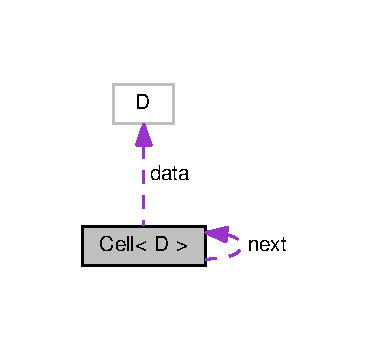
\includegraphics[width=178pt]{class_cell__coll__graph}
\end{center}
\end{figure}
\subsection*{Public Member Functions}
\begin{DoxyCompactItemize}
\item 
{\bf Cell} ()
\item 
{\bf Cell} (D $\ast$d, {\bf Cell} $\ast$c)
\item 
{\bfseries Cell} (const {\bf Cell} \&orig)\label{class_cell_a260a5d52d571c8d2f951d81df17154e2}

\end{DoxyCompactItemize}
\subsection*{Public Attributes}
\begin{DoxyCompactItemize}
\item 
{\bf Cell} $\ast$ {\bf next}\label{class_cell_a7e0e6c090f8aca70862c2dbc3257e3b9}

\begin{DoxyCompactList}\small\item\em Puntero que apunta a la celda siguiente. \end{DoxyCompactList}\item 
D $\ast$ {\bf data}\label{class_cell_ab8cc4d3059ef84a652eabc05b6c28f49}

\begin{DoxyCompactList}\small\item\em Puntero que apunta al dato almacenado en la celda. \end{DoxyCompactList}\end{DoxyCompactItemize}


\subsection{Detailed Description}
\subsubsection*{template$<$typename D$>$class Cell$<$ D $>$}

Plantilla de la clase Celda 

\subsection{Constructor \& Destructor Documentation}
\index{Cell@{Cell}!Cell@{Cell}}
\index{Cell@{Cell}!Cell@{Cell}}
\subsubsection[{Cell}]{\setlength{\rightskip}{0pt plus 5cm}template$<$typename D $>$ {\bf Cell}$<$ D $>$\-::{\bf Cell} (
\begin{DoxyParamCaption}
{}
\end{DoxyParamCaption}
)\hspace{0.3cm}{\ttfamily [inline]}}\label{class_cell_a742a2adf7fa420fa9cbe386a87b5c79b}
Constructor de la clase celda, sus atributos inician en nulo \index{Cell@{Cell}!Cell@{Cell}}
\index{Cell@{Cell}!Cell@{Cell}}
\subsubsection[{Cell}]{\setlength{\rightskip}{0pt plus 5cm}template$<$typename D $>$ {\bf Cell}$<$ D $>$\-::{\bf Cell} (
\begin{DoxyParamCaption}
\item[{D $\ast$}]{d, }
\item[{{\bf Cell}$<$ D $>$ $\ast$}]{c}
\end{DoxyParamCaption}
)\hspace{0.3cm}{\ttfamily [inline]}}\label{class_cell_aa8960323a8eeb23294419dd31349f18f}
Constructor de la clase celda, asigna a data y next, los valores recibidos como atributos 
\begin{DoxyParams}{Parameters}
{\em d} & puntero de tipo D \\
\hline
{\em c} & puntero de tipo \doxyref{Cell}{p.}{class_cell} \\
\hline
\end{DoxyParams}


The documentation for this class was generated from the following file\-:\begin{DoxyCompactItemize}
\item 
Cell.\-h\end{DoxyCompactItemize}

\section{Levenshtein Class Reference}
\label{class_levenshtein}\index{Levenshtein@{Levenshtein}}


Collaboration diagram for Levenshtein\-:\nopagebreak
\begin{figure}[H]
\begin{center}
\leavevmode
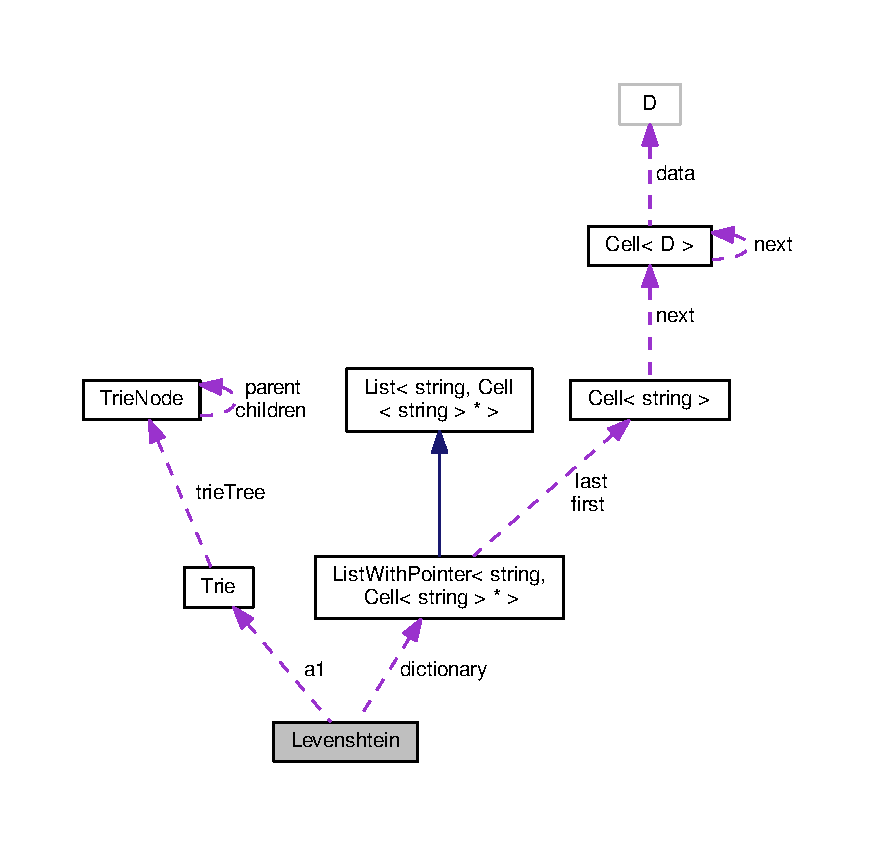
\includegraphics[width=194pt]{class_levenshtein__coll__graph}
\end{center}
\end{figure}
\subsection*{Public Member Functions}
\begin{DoxyCompactItemize}
\item 
{\bf Levenshtein} (int {\bf max\-Cost}, string file, string {\bf word})
\item 
{\bf List\-With\-Pointer}$<$ string, {\bf Cell}\\*
$<$ string $>$ $\ast$ $>$ $\ast$ {\bf Levenshtein\-Row} ()
\item 
int {\bf min} (int a, int b, int c)
\item 
void {\bf search\-Recursive} ({\bf Trie\-Node} $\ast$node, char letter, {\bf List\-With\-Pointer}$<$ int, {\bf Cell}$<$ int $>$ $\ast$ $>$ $\ast$prev\-Row, {\bf List\-With\-Pointer}$<$ string, {\bf Cell}$<$ string $>$ $\ast$ $>$ $\ast$result)
\item 
int {\bf Levenshtein\-\_\-alg} (string s1)
\item 
bool {\bf in\-Range} ({\bf Trie\-Node} $\ast$a)
\item 
{\bf List\-With\-Pointer}$<$ string, {\bf Cell}\\*
$<$ string $>$ $\ast$ $>$ $\ast$ {\bf Levenshtein\-Matrix} ({\bf Trie\-Node} $\ast$a)
\end{DoxyCompactItemize}
\subsection*{Public Attributes}
\begin{DoxyCompactItemize}
\item 
{\bf Trie} $\ast$ {\bf a1}
\item 
int {\bf max\-Cost}
\item 
string {\bf word}
\end{DoxyCompactItemize}


\subsection{Constructor \& Destructor Documentation}
\index{Levenshtein@{Levenshtein}!Levenshtein@{Levenshtein}}
\index{Levenshtein@{Levenshtein}!Levenshtein@{Levenshtein}}
\subsubsection[{Levenshtein}]{\setlength{\rightskip}{0pt plus 5cm}Levenshtein\-::\-Levenshtein (
\begin{DoxyParamCaption}
\item[{int}]{max\-Cost, }
\item[{string}]{file, }
\item[{string}]{word}
\end{DoxyParamCaption}
)}\label{class_levenshtein_aa896d5d6920c0457cf5591e5ddfb4605}
Constructor de la clase \doxyref{Levenshtein}{p.}{class_levenshtein}. 
\begin{DoxyParams}{Parameters}
{\em max\-Cost} & mayor distancia permitida entre palabras \\
\hline
{\em file} & archivo en el cual se van a buscar las coincidencias. \\
\hline
{\em word} & palabra a la cual se le quiere encontrar coincidencias dentro del archivo. \\
\hline
\end{DoxyParams}


\subsection{Member Function Documentation}
\index{Levenshtein@{Levenshtein}!in\-Range@{in\-Range}}
\index{in\-Range@{in\-Range}!Levenshtein@{Levenshtein}}
\subsubsection[{in\-Range}]{\setlength{\rightskip}{0pt plus 5cm}bool Levenshtein\-::in\-Range (
\begin{DoxyParamCaption}
\item[{{\bf Trie\-Node} $\ast$}]{a}
\end{DoxyParamCaption}
)}\label{class_levenshtein_aa1cb5956d10477a430a0a70662a1fe27}
Indica si la palabra cumple con el rango de caracteres necesarios, es decir, si la string que contiene a tiene un tamaño entre la cantidad de caracteres de la palabra + max\-Cost y la cantidad de caracteres de la palabra -\/ max\-Cost. 
\begin{DoxyParams}{Parameters}
{\em s1,string} & por comparar. \\
\hline
\end{DoxyParams}
\begin{DoxyReturn}{Returns}
true si si la cumple. 

false de lo contrario. 
\end{DoxyReturn}
\index{Levenshtein@{Levenshtein}!Levenshtein\-\_\-alg@{Levenshtein\-\_\-alg}}
\index{Levenshtein\-\_\-alg@{Levenshtein\-\_\-alg}!Levenshtein@{Levenshtein}}
\subsubsection[{Levenshtein\-\_\-alg}]{\setlength{\rightskip}{0pt plus 5cm}int Levenshtein\-::\-Levenshtein\-\_\-alg (
\begin{DoxyParamCaption}
\item[{string}]{s1}
\end{DoxyParamCaption}
)}\label{class_levenshtein_a11fa7f55b25f9782242c4b5f8d05bd7d}
Crea la matriz que indica la distancia entre la string s1 y la palabra buscada. 
\begin{DoxyParams}{Parameters}
{\em s1} & string a la cual se le va a sacar la distancia con respecto a word. \\
\hline
\end{DoxyParams}
\begin{DoxyReturn}{Returns}
distancia entre las palabras. 
\end{DoxyReturn}
\index{Levenshtein@{Levenshtein}!Levenshtein\-Matrix@{Levenshtein\-Matrix}}
\index{Levenshtein\-Matrix@{Levenshtein\-Matrix}!Levenshtein@{Levenshtein}}
\subsubsection[{Levenshtein\-Matrix}]{\setlength{\rightskip}{0pt plus 5cm}{\bf List\-With\-Pointer}$<$ string, {\bf Cell}$<$ string $>$ $\ast$ $>$ $\ast$ Levenshtein\-::\-Levenshtein\-Matrix (
\begin{DoxyParamCaption}
\item[{{\bf Trie\-Node} $\ast$}]{a}
\end{DoxyParamCaption}
)}\label{class_levenshtein_acc66dfa11af7a5e55d93d282a209554f}

\begin{DoxyItemize}
\item Este metodo recorre los nodos del árbol cuyo root es el nodo a. Es recursivo, pero solamente recorre los nodos que están en el rango para ser una coincidencia de acuerdo con el metodo \doxyref{in\-Range()}{p.}{class_levenshtein_aa1cb5956d10477a430a0a70662a1fe27} Para los nodos que son E\-O\-W, si tienen una distancia de \doxyref{Levenshtein}{p.}{class_levenshtein} menor o igual a la tolerancia (utilizando el metodo \doxyref{Levenshtein\-\_\-alg()}{p.}{class_levenshtein_a11fa7f55b25f9782242c4b5f8d05bd7d} ) se agregan a la lista lista\-Coincid. 
\begin{DoxyParams}{Parameters}
{\em a} & nodo en el que se encuentra. \\
\hline
\end{DoxyParams}
\begin{DoxyReturn}{Returns}
arreglo que contiene las coincidencias dentro del archivo. 
\end{DoxyReturn}

\end{DoxyItemize}\index{Levenshtein@{Levenshtein}!Levenshtein\-Row@{Levenshtein\-Row}}
\index{Levenshtein\-Row@{Levenshtein\-Row}!Levenshtein@{Levenshtein}}
\subsubsection[{Levenshtein\-Row}]{\setlength{\rightskip}{0pt plus 5cm}{\bf List\-With\-Pointer}$<$ string, {\bf Cell}$<$ string $>$ $\ast$ $>$ $\ast$ Levenshtein\-::\-Levenshtein\-Row (
\begin{DoxyParamCaption}
{}
\end{DoxyParamCaption}
)}\label{class_levenshtein_ada76c099240f39f30ddea66838457f48}
Este método crea una fila, que corresponde a la primera fila de la matriz = 0,1,2,.. hasta llegar al tamaño de la palabra buscada. Y llama al método search\-Recursive, que toma como prev\-Row esta fila y como nodo a los hijos de la raiz del trie. \begin{DoxyReturn}{Returns}
results arreglo que contiene todas las coincidencias dentro del archivo.$\ast$ 
\end{DoxyReturn}
\index{Levenshtein@{Levenshtein}!min@{min}}
\index{min@{min}!Levenshtein@{Levenshtein}}
\subsubsection[{min}]{\setlength{\rightskip}{0pt plus 5cm}int Levenshtein\-::min (
\begin{DoxyParamCaption}
\item[{int}]{a, }
\item[{int}]{b, }
\item[{int}]{c}
\end{DoxyParamCaption}
)}\label{class_levenshtein_a9d2b5ce5ae0292dad55f8ac600b221ae}
Da el valor minimo entre 3 enteros. \begin{DoxyReturn}{Returns}
valor minimo 
\end{DoxyReturn}
\index{Levenshtein@{Levenshtein}!search\-Recursive@{search\-Recursive}}
\index{search\-Recursive@{search\-Recursive}!Levenshtein@{Levenshtein}}
\subsubsection[{search\-Recursive}]{\setlength{\rightskip}{0pt plus 5cm}void Levenshtein\-::search\-Recursive (
\begin{DoxyParamCaption}
\item[{{\bf Trie\-Node} $\ast$}]{node, }
\item[{char}]{letter, }
\item[{{\bf List\-With\-Pointer}$<$ int, {\bf Cell}$<$ int $>$ $\ast$ $>$ $\ast$}]{prev\-Row, }
\item[{{\bf List\-With\-Pointer}$<$ string, {\bf Cell}$<$ string $>$ $\ast$ $>$ $\ast$}]{result}
\end{DoxyParamCaption}
)}\label{class_levenshtein_a6d7f860c3c07f37009f26ea1ab391cb8}
Se encarga de recorrer el árbol, nodo por nodo, de manera que se va creando un arreglo por punteros que indica la distancia entre la palabra y el string obtenido en el nodo. De tal forma, si aún existe una posibilidad de que el o los nodos hijos de dicho nodo contengan una palabra que esté en el rango de la distancia permitida, necesita únicamente el arreglo de la string analizada previamente y un arreglo por punteros nuevo para obtener la distancia de la nueva string, en vez de crear una matriz entera por cada palabra nueva. 
\begin{DoxyParams}{Parameters}
{\em node} & indica el nodo dentro del trie en el que se está buscando \\
\hline
{\em letter} & indica la letra que contiene dicho nodo. \\
\hline
{\em prev\-Row} & análisis de distancia del string que contiene el nodo padre. \\
\hline
{\em result} & arreglo que contiene las coincidencias encontradas. \\
\hline
\end{DoxyParams}


\subsection{Member Data Documentation}
\index{Levenshtein@{Levenshtein}!a1@{a1}}
\index{a1@{a1}!Levenshtein@{Levenshtein}}
\subsubsection[{a1}]{\setlength{\rightskip}{0pt plus 5cm}{\bf Trie}$\ast$ Levenshtein\-::a1}\label{class_levenshtein_acf70b2763312e65fb453b4c5b2adfa5d}
Objeto de tipo trie, donde se almacenan las palabras del archivo. \index{Levenshtein@{Levenshtein}!max\-Cost@{max\-Cost}}
\index{max\-Cost@{max\-Cost}!Levenshtein@{Levenshtein}}
\subsubsection[{max\-Cost}]{\setlength{\rightskip}{0pt plus 5cm}int Levenshtein\-::max\-Cost}\label{class_levenshtein_aefd28eb150c7d3baf3448551d18f9c9d}
Parámetro que indica la mayor distancia permitida entre palabras \index{Levenshtein@{Levenshtein}!word@{word}}
\index{word@{word}!Levenshtein@{Levenshtein}}
\subsubsection[{word}]{\setlength{\rightskip}{0pt plus 5cm}string Levenshtein\-::word}\label{class_levenshtein_ae0f3d52b4b02545b63e94509e0df0a85}
Palabra a la cual se le quiere encontrar coincidencias con una distancia menor a max\-Cost dentro del archivo 

The documentation for this class was generated from the following files\-:\begin{DoxyCompactItemize}
\item 
Levenshtein.\-h\item 
Levenshtein.\-cpp\end{DoxyCompactItemize}

\hypertarget{class_list}{\section{Referencia de la plantilla de la Clase List$<$ D, P $>$}
\label{class_list}\index{List$<$ D, P $>$@{List$<$ D, P $>$}}
}


{\ttfamily \#include $<$List.\-h$>$}



Diagrama de herencias de List$<$ D, P $>$\nopagebreak
\begin{figure}[H]
\begin{center}
\leavevmode
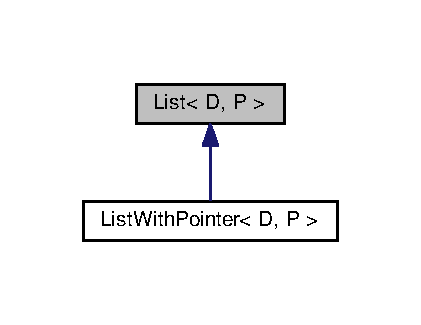
\includegraphics[width=202pt]{class_list__inherit__graph}
\end{center}
\end{figure}
\subsection*{Métodos públicos}
\begin{DoxyCompactItemize}
\item 
\hyperlink{class_list_a3deb54ab4f51c6c39aa4015f258b5812}{List} ()
\item 
\hyperlink{class_list_ad4d8108cecffb02dbc5e5e48691a0d43}{List} (int t)
\item 
\hyperlink{class_list_af8bcd7dae1bc30af2158075482c3d8d9}{List} (const \hyperlink{class_list}{List} \&orig)
\item 
virtual \hyperlink{class_list_a624593fb77847bf7ad4cacfba3442471}{$\sim$\-List} ()
\item 
virtual void \hyperlink{class_list_a01f588d87d47f8332928eca38f7b11bb}{insert} (D d)=0
\item 
virtual void \hyperlink{class_list_a14fc4e853102018df78db3899aa00d71}{remove} (D d)=0
\item 
virtual P \hyperlink{class_list_a2b40d6fffc7b2fb5138b648f52c839ee}{find} (D d)=0
\item 
virtual D \hyperlink{class_list_a5bd565e668247ae0691983227367cc88}{get} (P k)=0
\item 
virtual void \hyperlink{class_list_acb062aa988f4048498b30a2d845a311b}{assign} (P k, D d)=0
\item 
virtual void \hyperlink{class_list_ae3795939f27cf3e688cd470450e0c27a}{sort} ()=0
\item 
virtual int \hyperlink{class_list_af213bbcf13ee436a0f04cde66e337672}{get\-Size} ()=0
\item 
virtual void \hyperlink{class_list_a8b34931e187e7e6b86aad86510ce4f3b}{print\-List} ()=0
\item 
virtual P \hyperlink{class_list_a4ec3e88e176bb45bc49b030d1c8abb3f}{next} (P k)=0
\item 
virtual P \hyperlink{class_list_acc1831ae92a288345ef20cb29f3846b2}{prev} (P k)=0
\item 
virtual void \hyperlink{class_list_a24b4f177a70215980e81ef7b2981fa1e}{empty\-List} ()=0
\end{DoxyCompactItemize}


\subsection{Descripción detallada}
\subsubsection*{template$<$typename D, typename P$>$class List$<$ D, P $>$}

Plantilla de la clase \hyperlink{class_list}{List} 

\subsection{Documentación del constructor y destructor}
\hypertarget{class_list_a3deb54ab4f51c6c39aa4015f258b5812}{\index{List@{List}!List@{List}}
\index{List@{List}!List@{List}}
\subsubsection[{List}]{\setlength{\rightskip}{0pt plus 5cm}template$<$typename D, typename P$>$ {\bf List}$<$ D, P $>$\-::{\bf List} (
\begin{DoxyParamCaption}
{}
\end{DoxyParamCaption}
)\hspace{0.3cm}{\ttfamily [inline]}}}\label{class_list_a3deb54ab4f51c6c39aa4015f258b5812}
Constructor de la clase Lista sin atributos \hypertarget{class_list_ad4d8108cecffb02dbc5e5e48691a0d43}{\index{List@{List}!List@{List}}
\index{List@{List}!List@{List}}
\subsubsection[{List}]{\setlength{\rightskip}{0pt plus 5cm}template$<$typename D, typename P$>$ {\bf List}$<$ D, P $>$\-::{\bf List} (
\begin{DoxyParamCaption}
\item[{int}]{t}
\end{DoxyParamCaption}
)\hspace{0.3cm}{\ttfamily [inline]}}}\label{class_list_ad4d8108cecffb02dbc5e5e48691a0d43}
Constructor de la clase Lista. 
\begin{DoxyParams}{Parámetros}
{\em t} & tamaño de la lista \\
\hline
\end{DoxyParams}
\hypertarget{class_list_af8bcd7dae1bc30af2158075482c3d8d9}{\index{List@{List}!List@{List}}
\index{List@{List}!List@{List}}
\subsubsection[{List}]{\setlength{\rightskip}{0pt plus 5cm}template$<$typename D, typename P$>$ {\bf List}$<$ D, P $>$\-::{\bf List} (
\begin{DoxyParamCaption}
\item[{const {\bf List}$<$ D, P $>$ \&}]{orig}
\end{DoxyParamCaption}
)\hspace{0.3cm}{\ttfamily [inline]}}}\label{class_list_af8bcd7dae1bc30af2158075482c3d8d9}
Constructor por copia \hypertarget{class_list_a624593fb77847bf7ad4cacfba3442471}{\index{List@{List}!$\sim$\-List@{$\sim$\-List}}
\index{$\sim$\-List@{$\sim$\-List}!List@{List}}
\subsubsection[{$\sim$\-List}]{\setlength{\rightskip}{0pt plus 5cm}template$<$typename D, typename P$>$ virtual {\bf List}$<$ D, P $>$\-::$\sim${\bf List} (
\begin{DoxyParamCaption}
{}
\end{DoxyParamCaption}
)\hspace{0.3cm}{\ttfamily [inline]}, {\ttfamily [virtual]}}}\label{class_list_a624593fb77847bf7ad4cacfba3442471}
Destructor de la clase lista 

\subsection{Documentación de las funciones miembro}
\hypertarget{class_list_acb062aa988f4048498b30a2d845a311b}{\index{List@{List}!assign@{assign}}
\index{assign@{assign}!List@{List}}
\subsubsection[{assign}]{\setlength{\rightskip}{0pt plus 5cm}template$<$typename D, typename P$>$ virtual void {\bf List}$<$ D, P $>$\-::assign (
\begin{DoxyParamCaption}
\item[{P}]{k, }
\item[{D}]{d}
\end{DoxyParamCaption}
)\hspace{0.3cm}{\ttfamily [pure virtual]}}}\label{class_list_acb062aa988f4048498b30a2d845a311b}
Metodo virtual assign, asigna a una determinada posicion k, el valor d 
\begin{DoxyParams}{Parámetros}
{\em k} & dato tipo P, es una posicion o celda. \\
\hline
{\em d} & dado tipo D, que se quiere asignar a k \\
\hline
\end{DoxyParams}


Implementado en \hyperlink{class_list_with_pointer_aeaa834b22c4d7276a77ff29df3da7a30}{List\-With\-Pointer$<$ D, P $>$} y \hyperlink{class_list_with_pointer_aeaa834b22c4d7276a77ff29df3da7a30}{List\-With\-Pointer$<$ string, Cell$<$ string $>$ $\ast$ $>$}.

\hypertarget{class_list_a24b4f177a70215980e81ef7b2981fa1e}{\index{List@{List}!empty\-List@{empty\-List}}
\index{empty\-List@{empty\-List}!List@{List}}
\subsubsection[{empty\-List}]{\setlength{\rightskip}{0pt plus 5cm}template$<$typename D, typename P$>$ virtual void {\bf List}$<$ D, P $>$\-::empty\-List (
\begin{DoxyParamCaption}
{}
\end{DoxyParamCaption}
)\hspace{0.3cm}{\ttfamily [pure virtual]}}}\label{class_list_a24b4f177a70215980e81ef7b2981fa1e}
Metodo empty\-List, vacia la lista 

Implementado en \hyperlink{class_list_with_pointer_aec4f5374971962c79d397bbcd0080199}{List\-With\-Pointer$<$ D, P $>$} y \hyperlink{class_list_with_pointer_aec4f5374971962c79d397bbcd0080199}{List\-With\-Pointer$<$ string, Cell$<$ string $>$ $\ast$ $>$}.

\hypertarget{class_list_a2b40d6fffc7b2fb5138b648f52c839ee}{\index{List@{List}!find@{find}}
\index{find@{find}!List@{List}}
\subsubsection[{find}]{\setlength{\rightskip}{0pt plus 5cm}template$<$typename D, typename P$>$ virtual P {\bf List}$<$ D, P $>$\-::find (
\begin{DoxyParamCaption}
\item[{D}]{d}
\end{DoxyParamCaption}
)\hspace{0.3cm}{\ttfamily [pure virtual]}}}\label{class_list_a2b40d6fffc7b2fb5138b648f52c839ee}
Metodo virtual find, busca dentro de la lista el dato d. 
\begin{DoxyParams}{Parámetros}
{\em d} & dato tipo D que se desea encontrar. \\
\hline
\end{DoxyParams}
\begin{DoxyReturn}{Devuelve}
posicion o celda donde se encuentra el dato 
\end{DoxyReturn}


Implementado en \hyperlink{class_list_with_pointer_afeff8b963c197378553e2a3f73eaf66a}{List\-With\-Pointer$<$ D, P $>$} y \hyperlink{class_list_with_pointer_afeff8b963c197378553e2a3f73eaf66a}{List\-With\-Pointer$<$ string, Cell$<$ string $>$ $\ast$ $>$}.

\hypertarget{class_list_a5bd565e668247ae0691983227367cc88}{\index{List@{List}!get@{get}}
\index{get@{get}!List@{List}}
\subsubsection[{get}]{\setlength{\rightskip}{0pt plus 5cm}template$<$typename D, typename P$>$ virtual D {\bf List}$<$ D, P $>$\-::get (
\begin{DoxyParamCaption}
\item[{P}]{k}
\end{DoxyParamCaption}
)\hspace{0.3cm}{\ttfamily [pure virtual]}}}\label{class_list_a5bd565e668247ae0691983227367cc88}
Metodo virtual get, da el valor que se encuentra almacenado en la posicion k. 
\begin{DoxyParams}{Parámetros}
{\em k} & dato tipo P, es una posicion o celda. \\
\hline
\end{DoxyParams}
\begin{DoxyReturn}{Devuelve}
retorna el valor almacenado en k 
\end{DoxyReturn}


Implementado en \hyperlink{class_list_with_pointer_a0ff36c852334da8bc167356e636c1846}{List\-With\-Pointer$<$ D, P $>$} y \hyperlink{class_list_with_pointer_a0ff36c852334da8bc167356e636c1846}{List\-With\-Pointer$<$ string, Cell$<$ string $>$ $\ast$ $>$}.

\hypertarget{class_list_af213bbcf13ee436a0f04cde66e337672}{\index{List@{List}!get\-Size@{get\-Size}}
\index{get\-Size@{get\-Size}!List@{List}}
\subsubsection[{get\-Size}]{\setlength{\rightskip}{0pt plus 5cm}template$<$typename D, typename P$>$ virtual int {\bf List}$<$ D, P $>$\-::get\-Size (
\begin{DoxyParamCaption}
{}
\end{DoxyParamCaption}
)\hspace{0.3cm}{\ttfamily [pure virtual]}}}\label{class_list_af213bbcf13ee436a0f04cde66e337672}
Metodo virtual get\-Size, da el tamaño de la lista. \begin{DoxyReturn}{Devuelve}
el tamaño de la lista 
\end{DoxyReturn}


Implementado en \hyperlink{class_list_with_pointer_ac70c49b5703887fd867e90cdac3c706f}{List\-With\-Pointer$<$ D, P $>$} y \hyperlink{class_list_with_pointer_ac70c49b5703887fd867e90cdac3c706f}{List\-With\-Pointer$<$ string, Cell$<$ string $>$ $\ast$ $>$}.

\hypertarget{class_list_a01f588d87d47f8332928eca38f7b11bb}{\index{List@{List}!insert@{insert}}
\index{insert@{insert}!List@{List}}
\subsubsection[{insert}]{\setlength{\rightskip}{0pt plus 5cm}template$<$typename D, typename P$>$ virtual void {\bf List}$<$ D, P $>$\-::insert (
\begin{DoxyParamCaption}
\item[{D}]{d}
\end{DoxyParamCaption}
)\hspace{0.3cm}{\ttfamily [pure virtual]}}}\label{class_list_a01f588d87d47f8332928eca38f7b11bb}
Metodo virtual insert, agrega el dato d a la lista. 
\begin{DoxyParams}{Parámetros}
{\em d} & dato tipo D que se desea agregar a la lista \\
\hline
\end{DoxyParams}


Implementado en \hyperlink{class_list_with_pointer_a676e57683ade8e179e8eff5885f7309a}{List\-With\-Pointer$<$ D, P $>$} y \hyperlink{class_list_with_pointer_a676e57683ade8e179e8eff5885f7309a}{List\-With\-Pointer$<$ string, Cell$<$ string $>$ $\ast$ $>$}.

\hypertarget{class_list_a4ec3e88e176bb45bc49b030d1c8abb3f}{\index{List@{List}!next@{next}}
\index{next@{next}!List@{List}}
\subsubsection[{next}]{\setlength{\rightskip}{0pt plus 5cm}template$<$typename D, typename P$>$ virtual P {\bf List}$<$ D, P $>$\-::next (
\begin{DoxyParamCaption}
\item[{P}]{k}
\end{DoxyParamCaption}
)\hspace{0.3cm}{\ttfamily [pure virtual]}}}\label{class_list_a4ec3e88e176bb45bc49b030d1c8abb3f}
Metodo next, da la posicion o celda que le sigue a k 
\begin{DoxyParams}{Parámetros}
{\em k} & dato tipo P, es una posicion o celda. \\
\hline
\end{DoxyParams}
\begin{DoxyReturn}{Devuelve}
la posicion siguiente a k 
\end{DoxyReturn}


Implementado en \hyperlink{class_list_with_pointer_a518b5ee89e3ad32ae7cd4ddd5d4fa7e9}{List\-With\-Pointer$<$ D, P $>$} y \hyperlink{class_list_with_pointer_a518b5ee89e3ad32ae7cd4ddd5d4fa7e9}{List\-With\-Pointer$<$ string, Cell$<$ string $>$ $\ast$ $>$}.

\hypertarget{class_list_acc1831ae92a288345ef20cb29f3846b2}{\index{List@{List}!prev@{prev}}
\index{prev@{prev}!List@{List}}
\subsubsection[{prev}]{\setlength{\rightskip}{0pt plus 5cm}template$<$typename D, typename P$>$ virtual P {\bf List}$<$ D, P $>$\-::prev (
\begin{DoxyParamCaption}
\item[{P}]{k}
\end{DoxyParamCaption}
)\hspace{0.3cm}{\ttfamily [pure virtual]}}}\label{class_list_acc1831ae92a288345ef20cb29f3846b2}
Metodo next, retorna la posicion o celda que precede a k 
\begin{DoxyParams}{Parámetros}
{\em k} & dato tipo P, es una posicion o celda. \\
\hline
\end{DoxyParams}
\begin{DoxyReturn}{Devuelve}
la posicion previa a k 
\end{DoxyReturn}


Implementado en \hyperlink{class_list_with_pointer_a7242068fcc3a193f0f7e94517856e431}{List\-With\-Pointer$<$ D, P $>$} y \hyperlink{class_list_with_pointer_a7242068fcc3a193f0f7e94517856e431}{List\-With\-Pointer$<$ string, Cell$<$ string $>$ $\ast$ $>$}.

\hypertarget{class_list_a8b34931e187e7e6b86aad86510ce4f3b}{\index{List@{List}!print\-List@{print\-List}}
\index{print\-List@{print\-List}!List@{List}}
\subsubsection[{print\-List}]{\setlength{\rightskip}{0pt plus 5cm}template$<$typename D, typename P$>$ virtual void {\bf List}$<$ D, P $>$\-::print\-List (
\begin{DoxyParamCaption}
{}
\end{DoxyParamCaption}
)\hspace{0.3cm}{\ttfamily [pure virtual]}}}\label{class_list_a8b34931e187e7e6b86aad86510ce4f3b}
Metodo print\-List, imprime la lista 

Implementado en \hyperlink{class_list_with_pointer_a7079b5f1dbddb87a7e33ffc71ebb7b92}{List\-With\-Pointer$<$ D, P $>$} y \hyperlink{class_list_with_pointer_a7079b5f1dbddb87a7e33ffc71ebb7b92}{List\-With\-Pointer$<$ string, Cell$<$ string $>$ $\ast$ $>$}.

\hypertarget{class_list_a14fc4e853102018df78db3899aa00d71}{\index{List@{List}!remove@{remove}}
\index{remove@{remove}!List@{List}}
\subsubsection[{remove}]{\setlength{\rightskip}{0pt plus 5cm}template$<$typename D, typename P$>$ virtual void {\bf List}$<$ D, P $>$\-::remove (
\begin{DoxyParamCaption}
\item[{D}]{d}
\end{DoxyParamCaption}
)\hspace{0.3cm}{\ttfamily [pure virtual]}}}\label{class_list_a14fc4e853102018df78db3899aa00d71}
Metodo virtual remove , remueve el dato d de la lista, si este existe. 
\begin{DoxyParams}{Parámetros}
{\em d} & dato tipo D que se desea remover de la lista \\
\hline
\end{DoxyParams}


Implementado en \hyperlink{class_list_with_pointer_abcb151e95e9fffea7f9f7af593d8176f}{List\-With\-Pointer$<$ D, P $>$} y \hyperlink{class_list_with_pointer_abcb151e95e9fffea7f9f7af593d8176f}{List\-With\-Pointer$<$ string, Cell$<$ string $>$ $\ast$ $>$}.

\hypertarget{class_list_ae3795939f27cf3e688cd470450e0c27a}{\index{List@{List}!sort@{sort}}
\index{sort@{sort}!List@{List}}
\subsubsection[{sort}]{\setlength{\rightskip}{0pt plus 5cm}template$<$typename D, typename P$>$ virtual void {\bf List}$<$ D, P $>$\-::sort (
\begin{DoxyParamCaption}
{}
\end{DoxyParamCaption}
)\hspace{0.3cm}{\ttfamily [pure virtual]}}}\label{class_list_ae3795939f27cf3e688cd470450e0c27a}
Metodo virtual sort, ordena la lista 

Implementado en \hyperlink{class_list_with_pointer_aa46631b2da29895d1f767626fb591bc8}{List\-With\-Pointer$<$ D, P $>$} y \hyperlink{class_list_with_pointer_aa46631b2da29895d1f767626fb591bc8}{List\-With\-Pointer$<$ string, Cell$<$ string $>$ $\ast$ $>$}.



La documentación para esta clase fue generada a partir del siguiente fichero\-:\begin{DoxyCompactItemize}
\item 
List.\-h\end{DoxyCompactItemize}

\section{List\-With\-Pointer$<$ D, P $>$ Class Template Reference}
\label{class_list_with_pointer}\index{List\-With\-Pointer$<$ D, P $>$@{List\-With\-Pointer$<$ D, P $>$}}


{\ttfamily \#include $<$List\-With\-Pointer.\-h$>$}



Inheritance diagram for List\-With\-Pointer$<$ D, P $>$\-:\nopagebreak
\begin{figure}[H]
\begin{center}
\leavevmode
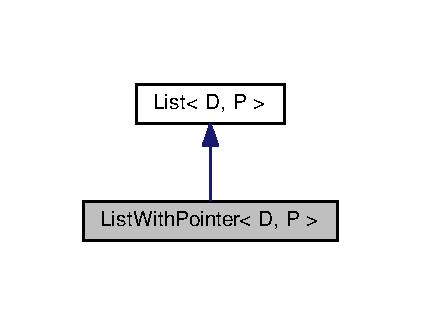
\includegraphics[width=202pt]{class_list_with_pointer__inherit__graph}
\end{center}
\end{figure}


Collaboration diagram for List\-With\-Pointer$<$ D, P $>$\-:\nopagebreak
\begin{figure}[H]
\begin{center}
\leavevmode
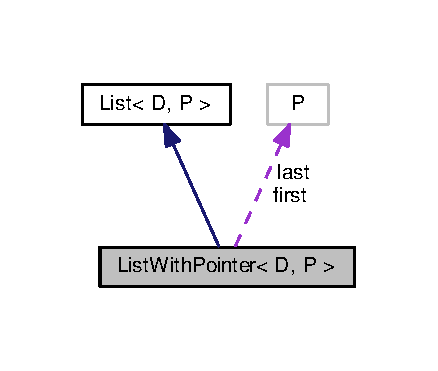
\includegraphics[width=202pt]{class_list_with_pointer__coll__graph}
\end{center}
\end{figure}
\subsection*{Public Member Functions}
\begin{DoxyCompactItemize}
\item 
{\bf List\-With\-Pointer} ()\label{class_list_with_pointer_a53b1284b13bf834bc5fc1eb27368a283}

\begin{DoxyCompactList}\small\item\em Constructor de la clase \doxyref{List\-With\-Pointer}{p.}{class_list_with_pointer}, los atributos first y null, son nulos y n es igual a cero. \end{DoxyCompactList}\item 
virtual {\bf $\sim$\-List\-With\-Pointer} ()\label{class_list_with_pointer_ac0567286c62e3521fa5130f95010e779}

\begin{DoxyCompactList}\small\item\em Destructor, elimina todos los elementos de la lista con \doxyref{empty\-List()}{p.}{class_list_with_pointer_aec4f5374971962c79d397bbcd0080199} \end{DoxyCompactList}\item 
void {\bf insert} (D d)
\begin{DoxyCompactList}\small\item\em Metodo insert. \end{DoxyCompactList}\item 
void {\bf remove} (D d)
\begin{DoxyCompactList}\small\item\em Metodo remove. \end{DoxyCompactList}\item 
P {\bf find} (D d)
\begin{DoxyCompactList}\small\item\em Metodo find. \end{DoxyCompactList}\item 
D {\bf get} (P k)
\begin{DoxyCompactList}\small\item\em Metodo get. \end{DoxyCompactList}\item 
void {\bf assign} (P k, D d)
\begin{DoxyCompactList}\small\item\em Metodo assign. \end{DoxyCompactList}\item 
void {\bf sort} ()
\begin{DoxyCompactList}\small\item\em Metodo sort. \end{DoxyCompactList}\item 
int {\bf get\-Size} ()
\begin{DoxyCompactList}\small\item\em Metodo get\-Size. \end{DoxyCompactList}\item 
void {\bf print\-List} ()
\begin{DoxyCompactList}\small\item\em Metodo print\-List. \end{DoxyCompactList}\item 
P {\bf next} (P k)
\begin{DoxyCompactList}\small\item\em Metodo next. \end{DoxyCompactList}\item 
P {\bf prev} (P k)
\begin{DoxyCompactList}\small\item\em Metodo previous. \end{DoxyCompactList}\item 
void {\bf empty\-List} ()
\begin{DoxyCompactList}\small\item\em Metodo empty\-List. \end{DoxyCompactList}\end{DoxyCompactItemize}
\subsection*{Public Attributes}
\begin{DoxyCompactItemize}
\item 
int {\bf n}\label{class_list_with_pointer_aac685c03cf811f155e2e0393a833ae33}

\begin{DoxyCompactList}\small\item\em Atributo de la clase que dice el tamaño de la lista. \end{DoxyCompactList}\item 
P {\bf first}\label{class_list_with_pointer_a10f9bcf73fcff6ca7fae28bec209bd20}

\begin{DoxyCompactList}\small\item\em Puntero de tipo celda que indica el primer elemento de la lista. \end{DoxyCompactList}\item 
P {\bf last}\label{class_list_with_pointer_aa4ff3f43dffeb524dc1cf3ac5dfdb415}

\begin{DoxyCompactList}\small\item\em Puntero de tipo celda que indica el ultimo elemento de la lista. \end{DoxyCompactList}\end{DoxyCompactItemize}


\subsection{Detailed Description}
\subsubsection*{template$<$typename D, typename P$>$class List\-With\-Pointer$<$ D, P $>$}

Plantilla de la clase Lista con Punteros, que hereda de la clase \doxyref{List}{p.}{class_list}. 

\subsection{Member Function Documentation}
\index{List\-With\-Pointer@{List\-With\-Pointer}!assign@{assign}}
\index{assign@{assign}!ListWithPointer@{List\-With\-Pointer}}
\subsubsection[{assign}]{\setlength{\rightskip}{0pt plus 5cm}template$<$typename D, typename P$>$ void {\bf List\-With\-Pointer}$<$ D, P $>$\-::assign (
\begin{DoxyParamCaption}
\item[{P}]{k, }
\item[{D}]{d}
\end{DoxyParamCaption}
)\hspace{0.3cm}{\ttfamily [inline]}, {\ttfamily [virtual]}}\label{class_list_with_pointer_aeaa834b22c4d7276a77ff29df3da7a30}


Metodo assign. 

Metodo para asignar a una celda existente en la lista, un valor especifico 
\begin{DoxyParams}{Parameters}
{\em k} & puntero tipo Celda. \\
\hline
{\em d} & dato tipo D, el cual se quiere asignar a la celda k. \\
\hline
\end{DoxyParams}


Implements {\bf List$<$ D, P $>$} \doxyref{}{p.}{class_list_acb062aa988f4048498b30a2d845a311b}.

\index{List\-With\-Pointer@{List\-With\-Pointer}!empty\-List@{empty\-List}}
\index{empty\-List@{empty\-List}!ListWithPointer@{List\-With\-Pointer}}
\subsubsection[{empty\-List}]{\setlength{\rightskip}{0pt plus 5cm}template$<$typename D, typename P$>$ void {\bf List\-With\-Pointer}$<$ D, P $>$\-::empty\-List (
\begin{DoxyParamCaption}
{}
\end{DoxyParamCaption}
)\hspace{0.3cm}{\ttfamily [inline]}, {\ttfamily [virtual]}}\label{class_list_with_pointer_aec4f5374971962c79d397bbcd0080199}


Metodo empty\-List. 

Metodo que se encarga de vaciar la lista. 

Implements {\bf List$<$ D, P $>$} \doxyref{}{p.}{class_list_a24b4f177a70215980e81ef7b2981fa1e}.

\index{List\-With\-Pointer@{List\-With\-Pointer}!find@{find}}
\index{find@{find}!ListWithPointer@{List\-With\-Pointer}}
\subsubsection[{find}]{\setlength{\rightskip}{0pt plus 5cm}template$<$typename D, typename P$>$ P {\bf List\-With\-Pointer}$<$ D, P $>$\-::find (
\begin{DoxyParamCaption}
\item[{D}]{d}
\end{DoxyParamCaption}
)\hspace{0.3cm}{\ttfamily [inline]}, {\ttfamily [virtual]}}\label{class_list_with_pointer_afeff8b963c197378553e2a3f73eaf66a}


Metodo find. 

Metodo de busqueda de un dato en la lista. 
\begin{DoxyParams}{Parameters}
{\em d} & dato tipo D que se desea buscar en la lista \\
\hline
\end{DoxyParams}
\begin{DoxyReturn}{Returns}
la celda en la cual se encuentra alojado el dato. 
\end{DoxyReturn}


Implements {\bf List$<$ D, P $>$} \doxyref{}{p.}{class_list_a2b40d6fffc7b2fb5138b648f52c839ee}.

\index{List\-With\-Pointer@{List\-With\-Pointer}!get@{get}}
\index{get@{get}!ListWithPointer@{List\-With\-Pointer}}
\subsubsection[{get}]{\setlength{\rightskip}{0pt plus 5cm}template$<$typename D, typename P$>$ D {\bf List\-With\-Pointer}$<$ D, P $>$\-::get (
\begin{DoxyParamCaption}
\item[{P}]{k}
\end{DoxyParamCaption}
)\hspace{0.3cm}{\ttfamily [inline]}, {\ttfamily [virtual]}}\label{class_list_with_pointer_a0ff36c852334da8bc167356e636c1846}


Metodo get. 

Metodo de obtencion del dato contenido en una celda 
\begin{DoxyParams}{Parameters}
{\em k} & puntero tipo Celda. \\
\hline
\end{DoxyParams}
\begin{DoxyReturn}{Returns}
Retorna el dato contenido en la celda. 
\end{DoxyReturn}


Implements {\bf List$<$ D, P $>$} \doxyref{}{p.}{class_list_a5bd565e668247ae0691983227367cc88}.

\index{List\-With\-Pointer@{List\-With\-Pointer}!get\-Size@{get\-Size}}
\index{get\-Size@{get\-Size}!ListWithPointer@{List\-With\-Pointer}}
\subsubsection[{get\-Size}]{\setlength{\rightskip}{0pt plus 5cm}template$<$typename D, typename P$>$ int {\bf List\-With\-Pointer}$<$ D, P $>$\-::get\-Size (
\begin{DoxyParamCaption}
{}
\end{DoxyParamCaption}
)\hspace{0.3cm}{\ttfamily [inline]}, {\ttfamily [virtual]}}\label{class_list_with_pointer_ac70c49b5703887fd867e90cdac3c706f}


Metodo get\-Size. 

Metodo que devuelve el tamaño de la lista \begin{DoxyReturn}{Returns}
tamaño. 
\end{DoxyReturn}


Implements {\bf List$<$ D, P $>$} \doxyref{}{p.}{class_list_af213bbcf13ee436a0f04cde66e337672}.

\index{List\-With\-Pointer@{List\-With\-Pointer}!insert@{insert}}
\index{insert@{insert}!ListWithPointer@{List\-With\-Pointer}}
\subsubsection[{insert}]{\setlength{\rightskip}{0pt plus 5cm}template$<$typename D, typename P$>$ void {\bf List\-With\-Pointer}$<$ D, P $>$\-::insert (
\begin{DoxyParamCaption}
\item[{D}]{d}
\end{DoxyParamCaption}
)\hspace{0.3cm}{\ttfamily [inline]}, {\ttfamily [virtual]}}\label{class_list_with_pointer_a676e57683ade8e179e8eff5885f7309a}


Metodo insert. 

Inserta elementos en la lista. Si la lista esta vacia, se crea la celda y se almacena el dato, los punteros first y last apuntan a dicha celda. De lo contrario, se crea la celda, se almacena el dato y se asigna el puntero last a la ultima celda agregada. Se hace la conexion entre la penultima celda y la ultima, mediante el atributo de la clase \doxyref{Cell}{p.}{class_cell}\-: next. Aumenta en uno a n. 
\begin{DoxyParams}{Parameters}
{\em d} & dato tipo D que se desea insertar en la lista. \\
\hline
{\em \doxyref{Cell}{p.}{class_cell}} & celda que se crea para almacenar el dato d. \\
\hline
\end{DoxyParams}


Implements {\bf List$<$ D, P $>$} \doxyref{}{p.}{class_list_a01f588d87d47f8332928eca38f7b11bb}.

\index{List\-With\-Pointer@{List\-With\-Pointer}!next@{next}}
\index{next@{next}!ListWithPointer@{List\-With\-Pointer}}
\subsubsection[{next}]{\setlength{\rightskip}{0pt plus 5cm}template$<$typename D, typename P$>$ P {\bf List\-With\-Pointer}$<$ D, P $>$\-::next (
\begin{DoxyParamCaption}
\item[{P}]{k}
\end{DoxyParamCaption}
)\hspace{0.3cm}{\ttfamily [inline]}, {\ttfamily [virtual]}}\label{class_list_with_pointer_a518b5ee89e3ad32ae7cd4ddd5d4fa7e9}


Metodo next. 

Metodo que dice la celda siguiente a una celda dada. 
\begin{DoxyParams}{Parameters}
{\em k} & puntero tipo celda. \\
\hline
\end{DoxyParams}
\begin{DoxyReturn}{Returns}
la celda siguiente a k. 
\end{DoxyReturn}


Implements {\bf List$<$ D, P $>$} \doxyref{}{p.}{class_list_a4ec3e88e176bb45bc49b030d1c8abb3f}.

\index{List\-With\-Pointer@{List\-With\-Pointer}!prev@{prev}}
\index{prev@{prev}!ListWithPointer@{List\-With\-Pointer}}
\subsubsection[{prev}]{\setlength{\rightskip}{0pt plus 5cm}template$<$typename D, typename P$>$ P {\bf List\-With\-Pointer}$<$ D, P $>$\-::prev (
\begin{DoxyParamCaption}
\item[{P}]{k}
\end{DoxyParamCaption}
)\hspace{0.3cm}{\ttfamily [inline]}, {\ttfamily [virtual]}}\label{class_list_with_pointer_a7242068fcc3a193f0f7e94517856e431}


Metodo previous. 

Metodo que dice la celda anterior a una celda dada. 
\begin{DoxyParams}{Parameters}
{\em k} & puntero tipo celda. \\
\hline
\end{DoxyParams}
\begin{DoxyReturn}{Returns}
la celda anterior a k. 
\end{DoxyReturn}


Implements {\bf List$<$ D, P $>$} \doxyref{}{p.}{class_list_acc1831ae92a288345ef20cb29f3846b2}.

\index{List\-With\-Pointer@{List\-With\-Pointer}!print\-List@{print\-List}}
\index{print\-List@{print\-List}!ListWithPointer@{List\-With\-Pointer}}
\subsubsection[{print\-List}]{\setlength{\rightskip}{0pt plus 5cm}template$<$typename D, typename P$>$ void {\bf List\-With\-Pointer}$<$ D, P $>$\-::print\-List (
\begin{DoxyParamCaption}
{}
\end{DoxyParamCaption}
)\hspace{0.3cm}{\ttfamily [inline]}, {\ttfamily [virtual]}}\label{class_list_with_pointer_a7079b5f1dbddb87a7e33ffc71ebb7b92}


Metodo print\-List. 

Metodo que imprime la lista. 

Implements {\bf List$<$ D, P $>$} \doxyref{}{p.}{class_list_a8b34931e187e7e6b86aad86510ce4f3b}.

\index{List\-With\-Pointer@{List\-With\-Pointer}!remove@{remove}}
\index{remove@{remove}!ListWithPointer@{List\-With\-Pointer}}
\subsubsection[{remove}]{\setlength{\rightskip}{0pt plus 5cm}template$<$typename D, typename P$>$ void {\bf List\-With\-Pointer}$<$ D, P $>$\-::remove (
\begin{DoxyParamCaption}
\item[{D}]{d}
\end{DoxyParamCaption}
)\hspace{0.3cm}{\ttfamily [inline]}, {\ttfamily [virtual]}}\label{class_list_with_pointer_abcb151e95e9fffea7f9f7af593d8176f}


Metodo remove. 

Remueve una celda de la lista. Se asegura que la lista no este vacia.\-De ser asi se crea un puntero temp tipo celda, que apunta a la celda que almacena el dato d. Si temp apunta a first, se cambia first a apuntar al siguiente valor de la lista. De lo contrario, se crea un puntero temp2 tipo celda que apunta al valor anterior a temp. Se realiza la conexion entre temp2, y la celda siguiente a temp. Se elimina temp. 
\begin{DoxyParams}{Parameters}
{\em d} & dato tipo D que se desea remover de la lista. \\
\hline
\end{DoxyParams}


Implements {\bf List$<$ D, P $>$} \doxyref{}{p.}{class_list_a14fc4e853102018df78db3899aa00d71}.

\index{List\-With\-Pointer@{List\-With\-Pointer}!sort@{sort}}
\index{sort@{sort}!ListWithPointer@{List\-With\-Pointer}}
\subsubsection[{sort}]{\setlength{\rightskip}{0pt plus 5cm}template$<$typename D, typename P$>$ void {\bf List\-With\-Pointer}$<$ D, P $>$\-::sort (
\begin{DoxyParamCaption}
{}
\end{DoxyParamCaption}
)\hspace{0.3cm}{\ttfamily [inline]}, {\ttfamily [virtual]}}\label{class_list_with_pointer_aa46631b2da29895d1f767626fb591bc8}


Metodo sort. 

Metodo para ordenar la lista de menor a mayor 

Implements {\bf List$<$ D, P $>$} \doxyref{}{p.}{class_list_ae3795939f27cf3e688cd470450e0c27a}.



The documentation for this class was generated from the following file\-:\begin{DoxyCompactItemize}
\item 
List\-With\-Pointer.\-h\end{DoxyCompactItemize}

\section{Trie Class Reference}
\label{class_trie}\index{Trie@{Trie}}


Collaboration diagram for Trie\-:\nopagebreak
\begin{figure}[H]
\begin{center}
\leavevmode
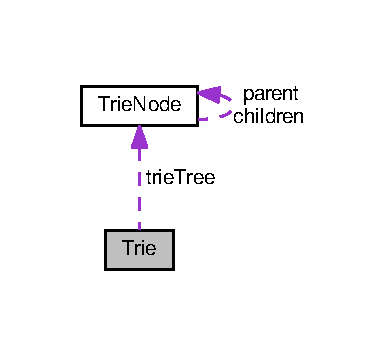
\includegraphics[width=187pt]{class_trie__coll__graph}
\end{center}
\end{figure}
\subsection*{Public Member Functions}
\begin{DoxyCompactItemize}
\item 
void {\bf create} (string text\-File)
\item 
void {\bf insert} (char $\ast$word)
\item 
{\bf Trie\-Node} $\ast$ {\bf search} (char $\ast$word)
\end{DoxyCompactItemize}
\subsection*{Public Attributes}
\begin{DoxyCompactItemize}
\item 
{\bf Trie\-Node} $\ast$ {\bf trie\-Tree}
\end{DoxyCompactItemize}


\subsection{Member Function Documentation}
\index{Trie@{Trie}!create@{create}}
\index{create@{create}!Trie@{Trie}}
\subsubsection[{create}]{\setlength{\rightskip}{0pt plus 5cm}void Trie\-::create (
\begin{DoxyParamCaption}
\item[{string}]{text\-File}
\end{DoxyParamCaption}
)}\label{class_trie_aba2fe23150879d718c56e51ab61006d4}
Crea el trie a partir de un archivo. Va leyendo línea por línea el archivo, y va insertando la palabra al trie. 
\begin{DoxyParams}{Parameters}
{\em text\-File} & archivo. \\
\hline
\end{DoxyParams}
\index{Trie@{Trie}!insert@{insert}}
\index{insert@{insert}!Trie@{Trie}}
\subsubsection[{insert}]{\setlength{\rightskip}{0pt plus 5cm}void Trie\-::insert (
\begin{DoxyParamCaption}
\item[{char $\ast$}]{word}
\end{DoxyParamCaption}
)}\label{class_trie_a5951beb416bb09f990126f5bc39aff58}
Inserta palabras en el trie. De manera que tiene un nodo current\-Node que se iguala a la raíz (trie\-Tree) y busca si current\-Node tiene un nodo hijo en la posición de la primera letra de la palabra, si no la tiene, crea un trie\-Node, de lo contrario current\-Node pasa a ser el nodo hijo y se continua con la siguiente letra de la palabra. 
\begin{DoxyParams}{Parameters}
{\em word} & palabra a insertar. \\
\hline
\end{DoxyParams}
\index{Trie@{Trie}!search@{search}}
\index{search@{search}!Trie@{Trie}}
\subsubsection[{search}]{\setlength{\rightskip}{0pt plus 5cm}{\bf Trie\-Node} $\ast$ Trie\-::search (
\begin{DoxyParamCaption}
\item[{char $\ast$}]{word}
\end{DoxyParamCaption}
)}\label{class_trie_ab9777dcdc2c9ccb8fe9080fa1a640109}
Busca si existe dentro del árbol la palabra word. Tiene un nodo current\-Node que inicia en el root del trie y se inicia con la primera letra de la palabra. Se ve si current\-Node tiene un trie\-Node (hijo) en la posición de la letra a buscar de children. De si tenerlo, current\-Node pasa a ser el nodo hijo y se continua con la siguiente letra de la palabra. Si se alcanza la última letra de la palabra, se verifica si E\-O\-W en dicho nodo es true. Si esto ocurre la palabra existe, de lo contrario no existe.


\begin{DoxyParams}{Parameters}
{\em word} & palabra buscada \\
\hline
\end{DoxyParams}
\begin{DoxyReturn}{Returns}
nodo donde se ubica la palabra. 
\end{DoxyReturn}


\subsection{Member Data Documentation}
\index{Trie@{Trie}!trie\-Tree@{trie\-Tree}}
\index{trie\-Tree@{trie\-Tree}!Trie@{Trie}}
\subsubsection[{trie\-Tree}]{\setlength{\rightskip}{0pt plus 5cm}{\bf Trie\-Node}$\ast$ Trie\-::trie\-Tree}\label{class_trie_a301aa208fe6fc7abaaf264c117070ed6}
Raíz del árbol 

The documentation for this class was generated from the following files\-:\begin{DoxyCompactItemize}
\item 
Trie.\-h\item 
Trie.\-cpp\end{DoxyCompactItemize}

\hypertarget{class_trie_node}{\section{Referencia de la Clase Trie\-Node}
\label{class_trie_node}\index{Trie\-Node@{Trie\-Node}}
}


Diagrama de colaboración para Trie\-Node\-:\nopagebreak
\begin{figure}[H]
\begin{center}
\leavevmode
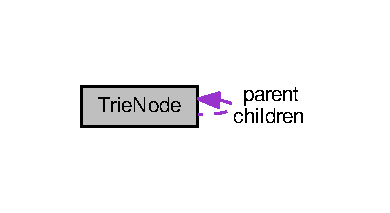
\includegraphics[width=187pt]{class_trie_node__coll__graph}
\end{center}
\end{figure}
\subsection*{Métodos públicos}
\begin{DoxyCompactItemize}
\item 
\hyperlink{class_trie_node_a3c44872f26b52fa29a38c91e69b22103}{Trie\-Node} ()
\item 
virtual \hyperlink{class_trie_node_a2c338a9960c601bbe654668cbe4f18a5}{$\sim$\-Trie\-Node} ()
\end{DoxyCompactItemize}
\subsection*{Atributos públicos}
\begin{DoxyCompactItemize}
\item 
\hyperlink{class_trie_node}{Trie\-Node} $\ast$ \hyperlink{class_trie_node_a523e346979214a75557e582fef02b3fd}{parent}
\item 
bool \hyperlink{class_trie_node_aeb4c2795d110df8c1fee5b494051e56d}{E\-O\-W}
\item 
\hyperlink{class_trie_node}{Trie\-Node} $\ast$ \hyperlink{class_trie_node_a3e37dd20032584eedaa6f45fda2b9698}{children} \mbox{[}A\-L\-P\-H\-A\-B\-E\-T\-\_\-\-S\-I\-Z\-E\mbox{]} = \{\}
\item 
string \hyperlink{class_trie_node_aa5fbf2d2487f8d1f3eecee4e8b999a16}{str}
\item 
int \hyperlink{class_trie_node_ae4cc4f53f8e5e06de5f460f6e8bbe0bb}{num\-Char}
\end{DoxyCompactItemize}


\subsection{Documentación del constructor y destructor}
\hypertarget{class_trie_node_a3c44872f26b52fa29a38c91e69b22103}{\index{Trie\-Node@{Trie\-Node}!Trie\-Node@{Trie\-Node}}
\index{Trie\-Node@{Trie\-Node}!TrieNode@{Trie\-Node}}
\subsubsection[{Trie\-Node}]{\setlength{\rightskip}{0pt plus 5cm}Trie\-Node\-::\-Trie\-Node (
\begin{DoxyParamCaption}
{}
\end{DoxyParamCaption}
)}}\label{class_trie_node_a3c44872f26b52fa29a38c91e69b22103}
Constructor de la clase \hyperlink{class_trie_node}{Trie\-Node} \hypertarget{class_trie_node_a2c338a9960c601bbe654668cbe4f18a5}{\index{Trie\-Node@{Trie\-Node}!$\sim$\-Trie\-Node@{$\sim$\-Trie\-Node}}
\index{$\sim$\-Trie\-Node@{$\sim$\-Trie\-Node}!TrieNode@{Trie\-Node}}
\subsubsection[{$\sim$\-Trie\-Node}]{\setlength{\rightskip}{0pt plus 5cm}Trie\-Node\-::$\sim$\-Trie\-Node (
\begin{DoxyParamCaption}
{}
\end{DoxyParamCaption}
)\hspace{0.3cm}{\ttfamily [virtual]}}}\label{class_trie_node_a2c338a9960c601bbe654668cbe4f18a5}
Destructor de la clase \hyperlink{class_trie_node}{Trie\-Node} 

\subsection{Documentación de los datos miembro}
\hypertarget{class_trie_node_a3e37dd20032584eedaa6f45fda2b9698}{\index{Trie\-Node@{Trie\-Node}!children@{children}}
\index{children@{children}!TrieNode@{Trie\-Node}}
\subsubsection[{children}]{\setlength{\rightskip}{0pt plus 5cm}{\bf Trie\-Node}$\ast$ Trie\-Node\-::children\mbox{[}A\-L\-P\-H\-A\-B\-E\-T\-\_\-\-S\-I\-Z\-E\mbox{]} = \{\}}}\label{class_trie_node_a3e37dd20032584eedaa6f45fda2b9698}
Corresponde a un arreglo de 26 caracteres en donde se crearan los nodos hijos de ese nodo. \hypertarget{class_trie_node_aeb4c2795d110df8c1fee5b494051e56d}{\index{Trie\-Node@{Trie\-Node}!E\-O\-W@{E\-O\-W}}
\index{E\-O\-W@{E\-O\-W}!TrieNode@{Trie\-Node}}
\subsubsection[{E\-O\-W}]{\setlength{\rightskip}{0pt plus 5cm}bool Trie\-Node\-::\-E\-O\-W}}\label{class_trie_node_aeb4c2795d110df8c1fee5b494051e56d}
Indica si existe una palabra \hypertarget{class_trie_node_ae4cc4f53f8e5e06de5f460f6e8bbe0bb}{\index{Trie\-Node@{Trie\-Node}!num\-Char@{num\-Char}}
\index{num\-Char@{num\-Char}!TrieNode@{Trie\-Node}}
\subsubsection[{num\-Char}]{\setlength{\rightskip}{0pt plus 5cm}int Trie\-Node\-::num\-Char}}\label{class_trie_node_ae4cc4f53f8e5e06de5f460f6e8bbe0bb}
Número de caracteres de la palabra que contiene el recorrido a dicho nodo. \hypertarget{class_trie_node_a523e346979214a75557e582fef02b3fd}{\index{Trie\-Node@{Trie\-Node}!parent@{parent}}
\index{parent@{parent}!TrieNode@{Trie\-Node}}
\subsubsection[{parent}]{\setlength{\rightskip}{0pt plus 5cm}{\bf Trie\-Node}$\ast$ Trie\-Node\-::parent}}\label{class_trie_node_a523e346979214a75557e582fef02b3fd}
Nodo que indica el nodo del que se generó dicho nodo. \hypertarget{class_trie_node_aa5fbf2d2487f8d1f3eecee4e8b999a16}{\index{Trie\-Node@{Trie\-Node}!str@{str}}
\index{str@{str}!TrieNode@{Trie\-Node}}
\subsubsection[{str}]{\setlength{\rightskip}{0pt plus 5cm}string Trie\-Node\-::str}}\label{class_trie_node_aa5fbf2d2487f8d1f3eecee4e8b999a16}
Palabra que contiene el recorrido a dicho nodo. 

La documentación para esta clase fue generada a partir de los siguientes ficheros\-:\begin{DoxyCompactItemize}
\item 
\hyperlink{_trie_node_8h}{Trie\-Node.\-h}\item 
\hyperlink{_trie_node_8cpp}{Trie\-Node.\-cpp}\end{DoxyCompactItemize}

%--- End generated contents ---

% Index
\newpage
\phantomsection
\addcontentsline{toc}{chapter}{Index}
\printindex

\end{document}
